\documentclass{article}

\usepackage{amsmath,amsthm}     
\usepackage{graphicx}     
\usepackage{hyperref} 
\usepackage{url}
\usepackage{amsfonts} 
\usepackage[margin=1in]{geometry}
\usepackage{float}
\usepackage{multicol, multirow}
\usepackage{arydshln}
\usepackage{subcaption}
\usepackage[french]{babel}
\usepackage{adjustbox}



\allowdisplaybreaks

\makeatletter
\@addtoreset{footnote}{page}
\makeatother

%%%%%%%%%%%%%%%%%%%%%%%%%%%%%%%%%%%%%%%%%%%%%%%%%%
\begin{document}

\renewcommand{\arraystretch}{1.5}

\title{BIML NLP : Classification d'émotions \\
\footnotesize{}}
\author{Bonhoure Timothé, Martinez Christophe}                      %%%% your final manuscript.

\maketitle
\tableofcontents
\section*{Abstract}
\newpage

\section{Modèle}
Notre architecture de modèle suit fidèlement les spécifications du sujet \ref{fig:modele_rnn}. Le processus commence par l'encodage en One Hot d'un mot en entrée, suivi d'un passage à travers une couche linéaire d'embedding. Par la suite, le modèle concatène la sortie de cette couche d'embedding avec des données cachées internes au modèle, permettant ainsi la mémorisation des mots précédents dans la phrase. Enfin, ces données sont traitées par deux couches en parallèle pour produire en sortie une classification de l'émotion associée à la phrase. De manière récurrente, les informations résultantes sont également réinjectées dans les données cachées pour le traitement du mot suivant. Toutes les couches sont des couches linéaires.

\begin{figure}[H]
    \centering
    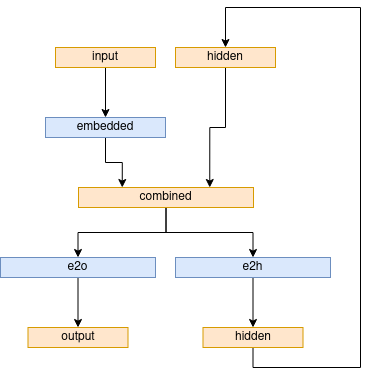
\includegraphics[width=0.4\linewidth]{img/modele.png}
    \caption{Modèle RNN}

    \label{fig:modele_rnn}
\end{figure}

\section{Entrainement}
La tâche principale de notre modèle consiste à classifier l'émotion associée à une phrase donnée. Pour entrainer notre modèle, nous avons choisi d'utiliser la fonction de perte \texttt{CrossEntropyLoss}. Cette fonction est largement adoptée dans les tâches de classification, en raison de sa capacité à inciter le modèle à être plus confiant dans ses prédictions. En effet, \texttt{CrossEntropyLoss} pénalise plus sévèrement les prédictions incorrectes associées à une forte confiance du modèle, favorisant ainsi une meilleure calibration des probabilités prédites. \\
Pour optimiser notre modèle, nous avons opté pour l'utilisation de l'optimiseur \texttt{AdamW}. Cette variante améliorée de l'optimiseur \texttt{Adam} intègre une correction spécifique pour la régularisation des poids, résolvant ainsi le problème de dégradation du poids associé à l'optimiseur \texttt{Adam} standard. 

\section{Préparation des données}
Nous avons décidé de ne conserver que les mots dont la fréquence d’apparition est de minimum 4. Nous estimons que cela équivaut à retirer environ 75\% des mots totaux de notre jeu de données en comptant les doublons. L’effet de ce filtrage a pour effet d’accélérer grandement l’entrainement de notre modèle. \\
En analysant la distribution des longueurs de phrases dans notre ensemble d'entraînement, nous constatons une longueur moyenne d'environ 20 mots avec une variance de 120. Ces statistiques guident notre choix de définir une longueur maximale de phrases à 15 mots pour notre modèle. \\
En plus de cela, nous recourons à la vectorisation TF-IDF pour chercher à extraire les caractéristiques de nos phrases en cherchant les mots les plus importants et significatifs. Parmi les 15 mots conservés de chaque phrase, nous avons préservé ceux présentant un meilleur score selon TF-IDF. \\
Ainsi préparé, notre jeu de données est prêt à être utilisé dans l'entraînement de notre modèle de classification d'émotions. Cette préparation tient compte de la fréquence des mots, de la longueur des phrases, et des caractéristiques TF-IDF significatives, pour tendre au maximum vers une représentation riche et pertinente pour la classification.

\section{Tâche secondaire}
Une couche supplémentaire a été incorporée en parallèle\ref{fig:modele_rnn_with_secondary} avec les deux précédentes pour accomplir une seconde tâche d'apprentissage basée sur la détection de la négation dans la phrase à classifier. Dans le cadre d'un prétraitement initial, les phrases ont été étiquetées manuellement comme étant négatives ou positives. Nous avons établi une liste de mots que nous considérons comme des indicateurs de négation, notamment "not", "n't", "never", "neither", "no", "none", "nobody", "nowhere", et "nothing". Ainsi, toute phrase contenant au moins l'un de ces mots est étiquetée comme négative pour l'apprentissage de notre modèle. \\
La tâche du modèle consiste désormais à prédire simultanément l'émotion associée à la phrase et à déterminer si la phrase est positive ou négative. Nous utilisons la fonction de perte \texttt{BCEWithLogitsLoss}, couramment utilisée pour la classification binaire. Dans notre cas, la classification de la phrase à travers cette tâche se résume à déterminer si la phrase est négative ou non. Ensuite, nous combinons cette perte avec la perte de la tâche principale en utilisant un poids préalablement défini afin d'évaluer une perte globale du modèle.

\begin{figure}[H]
    \centering
    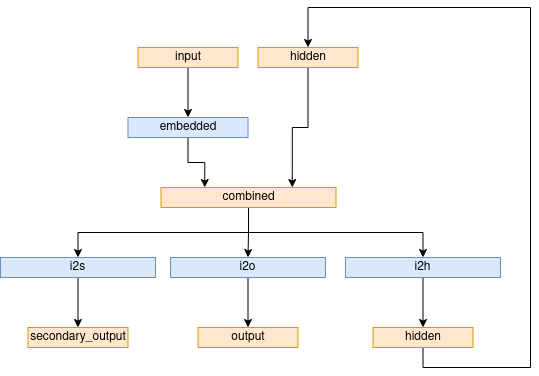
\includegraphics[width=0.5\linewidth]{img/modele_with_secondary.png}
    \caption{Modèle RNN avec tâche secondaire}

    \label{fig:modele_rnn_with_secondary}
\end{figure}

\section{Fonctionnalités développées}
Ainsi comme dit précédemment nous avons développé la classification d’émotion. Une tâche secondaire d’apprentissage par la négation. L’étude de la distribution des mots, le filtrage des mots rares et la recherche des mots portant le plus le sens avec TF-IDF.

\end{document}